\documentclass[a4paper, 12pt]{article}
\usepackage{pmgraph}
\usepackage[a4paper,portrait, margin=1.25in]{geometry}
\usepackage[normalem]{ulem}
\usepackage[swedish,english]{babel}
\usepackage{graphicx,here,times,tabularx,rotating}
\usepackage{multicol}
\usepackage{float}
\usepackage{amssymb}
\usepackage{amsthm}
\usepackage{amsmath}
\usepackage[bottom]{footmisc}
\usepackage{physics}
\usepackage{bbm}
\usepackage{gensymb}
\usepackage{hyperref}
\usepackage[export]{adjustbox}
\usepackage[nottoc]{tocbibind}
\usepackage[toc,page]{appendix}
\usepackage{lipsum}
\usepackage{framed,xcolor}
\usepackage{libertine}
\usepackage{algorithm2e}
\usepackage{bm}% bold math
\usepackage[utf8]{inputenc}
\usepackage{pgfplots}
\usepackage{tikz}
\usepackage{enumitem}
\usepackage{mathtools}
\usepackage{array}
\usetikzlibrary{arrows}
\usepackage{afterpage}





\newcommand{\HRule}{\rule{\linewidth}{0.5mm}} % Defines a new command for the horizontal lines, change thickness here
\newcommand{\note}[1]{{\color{red}\textbf{#1} } }


\newcommand{\inp}[2]{\langle #1,#2 \rangle}



\newcommand\blankpage{%
    \null
    \thispagestyle{empty}%
    \addtocounter{page}{-1}%
    \newpage}


\begin{document}

\pagenumbering{gobble}
%%%%%%%%%%%%%%%%%%%%%%%%%%%%%%%%%%%%%%%55
\begin{titlepage}


\center % Center everything on the page
 
 
 
 
%----------------------------------------------------------------------------------------
%	HEADING SECTIONS
%----------------------------------------------------------------------------------------

\textsc{\LARGE Uppsala University}\\[1.5cm] % Name of your university/college
\textsc{\Large Degree Project E in Computational Science, 30c}\\[0.5cm] % Major heading such as course name
\textsc{\large Department of Physics and Astronomy\\ Division of Materials Theory}\\[0.5cm] % Minor heading such as course title

%----------------------------------------------------------------------------------------
%	TITLE SECTION
%----------------------------------------------------------------------------------------

\HRule \\[0.4cm]
{ \huge \bfseries Holonomic Optimal Control for Qudits}\\[0.4cm] % Title of your document
\HRule \\[1.5cm]
 
%----------------------------------------------------------------------------------------
%	AUTHOR SECTION
%----------------------------------------------------------------------------------------

\begin{minipage}{0.4\textwidth}
\begin{flushleft} \large
\emph{Author:}\\
Tomas \textsc{André} % Your name
\end{flushleft}
\end{minipage}
~
\begin{minipage}{0.4\textwidth}
\begin{flushright} \large
\emph{Supervisor:} \\
Erik \textsc{Sjöqvist} \\
\emph{Subject reader:} \\
Martin \textsc{Almquist} %% Supervisor's Name
\end{flushright}
\end{minipage}\\[2cm]

% If you don't want a supervisor, uncomment the two lines below and remove the section above
%\Large \emph{Author:}\\
%John \textsc{Smith}\\[3cm] % Your name

%----------------------------------------------------------------------------------------
%	DATE SECTION
%----------------------------------------------------------------------------------------

{\large \today}\\[2cm] % Date, change the \today to a set date if you want to be precise

%----------------------------------------------------------------------------------------
%	LOGO SECTION
%----------------------------------------------------------------------------------------


\includegraphics[scale = 0.11]{figures/uulogga.png}\\[1cm] % Include a department/university logo - this will require the graphicx package
 
%----------------------------------------------------------------------------------------

\vfill % Fill the rest of the page with whitespace

\end{titlepage}
%%%%%%%%%%%%%%%%%%%%%%%%%%%%%%%%
\newpage\null\newpage % Intentional blankpage


\begin{abstract}
Non-adiabatic Holonomic Quantum Computation (NHQC) is a method used to implement quantum gates with holonomies that arise solely from non-Abelian geometric phases. Due to high noise tolerance these phases can be used to construct resiliant quantum gates. By using dark paths we show how to implement quantum gates for higher dimensional computation elements, qudits, instead of the conventional qubits. This gives higher parameter control compared to earlier implementations. We present a scheme that generalizes and achieves single-qudit universality using controllable high fidelity gates by including an auxiliary state. An explicit example is shown for the Qutrit. The scaling is linear in dimension and we show how any diagonal qudit gate can be implemented efficiently in any dimension.
\end{abstract}

\bigskip

\bigskip

\bigskip

\bigskip

\begin{otherlanguage}{swedish}
\begin{abstract}
Kvantmekaniska periodiska system uppvisar, förutom den väletablerade dynamiska fasen i tidsutveckligen, även en geometrisk fas. Eftersom denna fas är oberoende av systemets dynamik kan den användas för att skapa fel-toleranta kvantmekaniska grindar. Detta är grunden för s.k. Icke-adiabatic Holonomiska Kvantgrindar. Genom att utnyttja vägar i parameterrummet som inte bidrar med någon dynamisk utveckling så implementerar vi hög dimensionella beräkningselement, 'qudits', istället för de mer konvetionella kvantbitarna. Detta resulterar i högre kontroll över parameterar än vissa tidigare metoder. Vi visar hur detta schema kan generaliseras till högre dimensioner och hur man kan uppnå universalitet med dessa hög-dimensionella och fel-toleranta kvantgrindar. Ett exempel ges för tre dimensioner och används som grund som sedan generaliseras. Schemat har linjär skalning i dimension och diagonala qudit-grindar kan effektivt bli implementerade i höga dimensioner.
\end{abstract}
\end{otherlanguage}

\newpage\null\newpage % Intentional blankpage

\tableofcontents

\newpage\null\newpage % Intentional blankpage

\pagenumbering{arabic}

\section{Introduction}
The emerging field of quantum technology has many promising applications, one of them is quantum computation (QC), which currently is a very active area of research. Quantum computers make use of quantum mechanical effects such as superposition, entanglement, and interference to design powerful algorithms. These algorithms could be used to solve some hard problems which would not be  possible to solve using classical computation, such as efficient prime-number factoring [1]. It can also be used to reduce the time complexity of some commonly used algorithms [2]. Current quantum computers are very susceptible to decoherence and noise, and thus will not have any commercial use any time soon, but stand as an important proof of concept. 
The most common model for quantum computation is the circuit model, which is analogous to the classical circuits used for classical computers. Gates are replaced by unitary transformations (quantum gates) and bits by qubits. To achieve the computational advantage it is important to construct robust, noise-resilient quantum gates. A good candidate for this is holonomic quantum computation [3,4], which is based on the Berry phase [5] and its non-Abelian and/or non-adiabatic generalizations [6,7,8]. These methods are only dependent on the geometry of the system and thus are resilient to local errors in the dynamical evolution.


The idea that elements of computation should be limited to two-dimensional qubits is sort of an arbitrary choice that most likely rose out of convenience due to binary logic. So why binary logic? It is simply the easiest non-trivial example, in binary things can be either $1$ or $0$, {\tt True} or {\tt False}, \textbf{on} or \textbf{off}. Due to its simplicity, it is no wonder that this is how the first computer was designed. But are we limited to bits? As early as 1840 a mechanical trenary (three-valued logic) calculation device was built by Thomas Fowler [9], and in 1958 the first electronic trenary computer was built by the Soviet Union [10]. Even though it had many advantages over the binary computer it never saw the same widespread success. There is nothing in theory that forbids a higher dimensional computational basis, even more so when it comes to quantum computers, where the implementation of the elements of computation already surpasses the simplicity of \textbf{on} and \textbf{off}. There are promising qudit results that show potential [11,12,13], and in the review article [14] a good overview of the field is given and further research into the topic is encouraged.

In this report we will show how to find a new geometric phase based scheme to implement qudits which could be more efficient than some current ones by making use of dark paths for increased parameter control and auxiliary states for increased fidelity. We do this by generalizing the idea of the scheme from [15]. The report is structured as follows. The background section is split into two parts where the first part serves as a quick introduction to the most important aspects of quantum mechanics as well as the commonly used notation. Then follows a part more concerned with quantum computation, quantum information, and some of the more advanced quantum mechanical concepts that those are built upon. Then the main results are shown, first an explicit example for the qutrit and then how it generalizes in higher dimensions. The report ends with conclusions and a brief outlook.




\newpage

\section{Theoretical background}
The Background consists of a quick introduction to the most important quantum mechanical concepts and notation. Readers familiar with quantum mechanics may skip it. The second part explores the fundamentals of quantum computation and 

\subsection{Basic quantum mechanics, part I}
This part offers a quick introduction to the necessary  quantum mechanics for readers whom are not familiar with the subject. The section contains nothing relevant for later parts of the thesis and can be safely skipped. For a more complete introduction I suggest chapter 1 of Sakurai.

\subsubsection{Kets, Bras and Operators}
When talking about Quantum mechanics the term \textbf{quantum state}, or more likley just state, is mentioned a lot. A quantum mechanical state is represented by a \textbf{ket}, an complex-valued vector with either finite or infinite entries. Closely related to the ket is the \textbf{bra}, which is the corresponding vector to the ket in the dual space, or more simply, the hermitian conjugate of the ket, see Equation \ref{eq:ket}.
\begin{equation}
\label{eq:ket}
\ket{\psi} = \begin{pmatrix}
a_1 \\ a_2 \\ \vdots \\ a_n
\end{pmatrix},\;
\bra{\psi} = (\ket{\psi})^{\dagger} = (a_1^{*}, a_2^{*}, \dots, a_n^{*}),\; a_1,a_2,\dots,a_n \in \mathbb{C}
\end{equation} 
An arbitrary ket can be rewritten as a linear combination of its eigenkets that span the same space, $\ket{\psi} = \sum_i a_i\ket{i}$ The coefficient is know as the probability amplitude, and $|a_i|^2$ corresponds to the probability to find the state in the $i$th state. 
The inner product of two quantum states is simply written as 
$\bra{\varphi}\ket{\psi} = (\bra{\varphi}\ket{\psi})^\dagger \in \mathbb{C}$. 
An operator can act on a quantum state and corresponds to multiplication with a matrix, and will always yield a new state, ket. 
\begin{equation}
\hat{O}\ket{\psi} = \ket{\psi'}
\end{equation}
Operators are often written in terms of of kets and bras, for example and operator which takes the state $\ket{1}$ and returns the state $\ket{2}$ is written as
\begin{equation}
(\ket{2}\bra{1})\ket{1} = \ket{2}\bra{1}\ket{1} = \ket{2}(\bra{1}\ket{1}) = (\bra{1}\ket{1})\ket{2} = 1 \ket{2} = \ket{2}
\end{equation}
or a identity $2\times 2$ matrix would be
\begin{equation}
 \begin{pmatrix}
 1 & 0 \\ 0 & 1
 \end{pmatrix} = \ket{1}\bra{1} + \ket{2}\bra{2} 
\end{equation}
and so on. An operator for a physical measurable quantity is called an observable.

\subsubsection{Measurements and Observables and Uncertainty}
A quantum mechanical measurement ''breaks'' the superposition of a quantum states and shifts it into a eigenstate of the observable,
\begin{equation}
\ket{\psi} \longrightarrow \ket{i}
\end{equation}
the probability to find the $i$th eigenstate is $|a_i|^2$. 
In quantum mechanics the relation $AB - BA = 0$,where $A$ and $B$ are operators, does not generally hold. This is due to the uncommutative nature of quantum mechanics, it relates to uncertainty but it also required since it a can realize a more complex mathematical structure. The fact that matrices are non-commutative are not surprising, and since operators can be represented by matrices this should not be that confusing. 
To make it more concrete to which degree two operators commute one can define  the commutator on operators $A,B$ as $[A,B] = AB - BA$, which is zero for commuting operators and non-zero otherwise. 
Observables which don't commute are called incompatible observables, a well know pair of incompatible observables are position and momentum, $\mathbf{x}$ and $\mathbf{p}$, which can not be measured to arbitrary precision, this is due to the fact that $[\mathbf{x},\mathbf{p}] \neq 0$. So for two incompatible observables the general uncertainty the measurements will be limited by \note{uncertainty relation here.} 

\subsubsection{Time evolution and the Schrödinger equation}

\subsection{Quantum Computation and Quantum Information theory, part 2}

\subsubsection{The Qubit}
A classical bit is a binary system which, so it can occupy two states, either 0 or 1. So with $n$ bits there is $2^n$ possible states that can be represented, but only one at a time.

A qubit is a quantum state that is in a superposition of $\ket{0}$ and $\ket{1}$, so a general qubit would have the form
\begin{equation}
\label{eq:qubit}
\ket{\psi} = \alpha\ket{0} + \beta\ket{1},\,\alpha,\beta \in \mathbb{C},\, |\alpha|^2 + |\beta|^2 = 1.
\end{equation}
The qubit is no limited to 0 and 1, but can exist in a linear combination of those states. When a measurement is performed the qubit will collapse into $\ket{1}$ or $\ket{2}$ with probability $|\alpha|^2$ and $|\beta|^2$ respectively. A consequence of superposition is that $n$ qubits can represent $2^n$ states simultaneously.

The combined state of two qubits $\ket{\psi_1}$ and $\ket{\psi_2}$ is given by 
\begin{equation}
\ket{\psi_1} \otimes \ket{\psi_2} = (\alpha_1\ket{0} + \beta_1\ket{1})\otimes(\alpha_2\ket{0} + \beta_2\ket{1})
\end{equation}
the tensor product is often omitted and one would write $\ket{\psi_1} \otimes \ket{\psi_2} = \ket{\psi_1}\ket{\psi_2} = \ket{\psi_1, \psi_2}$.

Some of the common qubit gates are the Pauli gates $X,Y,Z$, the Hadamard gate $H$, and the T-gate $T$.





\subsubsection{Information stuff}

\subsubsection{Universal computation}

\subsubsection{Holonomic Quantum Computation}



\newpage
\section{Results}
\section{The Qutrit}
\subsection{Construction of the system}
In \cite{darkpath} a qubit is implemented by modifying the lambda system, adding an additional level, and an auxiliary state, effectively turning it into a tripod. 
The generalization to implement a qutrit is not trivial but it is clear that one extra ground state is required to make the computational basis larger. Another thing that is needed is to limit the number of dark states to one. The number of dark states is the difference of the number of excited states and the number of ground states\cite{lambda} (here the auxiliary state is \textbf{not} counted as a ground state). Therefore another excited state must be added as well. How these states are coupled is the hard part, we will see that the system given by the Hamiltonian
\begin{equation}
\label{eq:Ham}
H = \sum_{j = 1}^2 \sum_{i =j}^{3} \omega_{ij}\ket{i}\bra{e_j}  + \frac{\Omega_{a}(t)}{2}\ket{a}\bra{e_2}  +\,\text{h.c}
\end{equation}
which is shown in Figure \ref{fig:Ham}, will work.  It consists of two excited states, $\ket{e_1}, \ket{e_2}$, an auxiliary state $\ket{a}$ and the ground states $\ket{1}, \ket{2}, \ket{3}$ which 
makes up the computational basis of the qutrit. By changing the basis of the Hamiltonian, it can be rewritten as 
\begin{equation}
\label{eq:Hamd}
H_d = \sum_{j = 1}^2 \frac{\Omega_j(t)}{2}e^{-i\phi_j}\ket{b_j}\bra{e_j}  + \frac{\Omega_a(t)}{2}\ket{a}\bra{e_2}  +\,\text{h.c}
\end{equation} 
by a Morris-Shore transformation\cite{morris}. We call this new basis the dark state basis. To find this basis find a dark state to the original  Hamiltonian, an eigenstate with eigenvalue $0$, $H\ket{d} = 0$, then find two bright states, orthogonal to both $\ket{d}$ and each other. This basis can be parametrized with 4 angles, $\theta, \varphi, \chi, \xi$, the dark state is on the form $\ket{d} = \cos\theta\ket{1} + e^{i\chi}\sin\theta\cos\varphi\ket{2} + e^{i\xi}\sin\theta\sin\varphi\ket{3}$, additionally the two bright states are $\ket{b_1} = N_1 \left(-e^{i\xi}\sin\theta\sin\varphi\ket{1} + \cos\theta\ket{2} \right)$ and $\ket{b_2} = N_2 \left(\cos\theta\ket{1} +  e^{i\chi}\sin\theta\cos\varphi\ket{2} + \Lambda \ket{3}\right ) $, where $N_1, N_2$ are normalization factors and $\Lambda$ can be chosen such that $\bra{d}\ket{b_2} = 0$.

\begin{figure}[H]
\label{fig:Ham}
    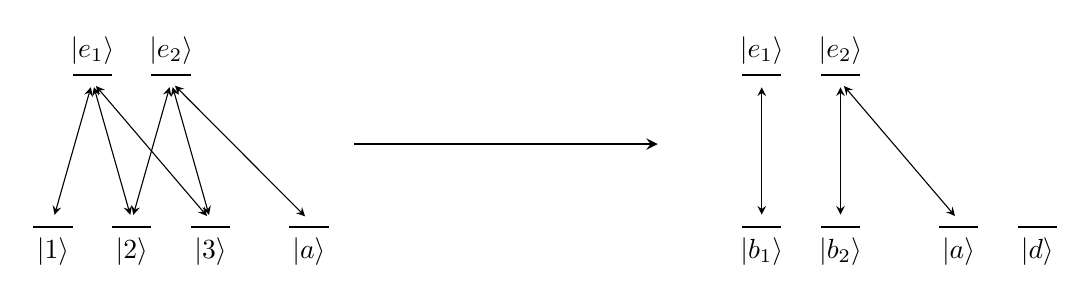
\begin{tikzpicture}[
      scale=0.5,
      level/.style={thick},
      virtual/.style={thick,densely dashed},
      trans/.style={thin,<->,shorten >=2pt,shorten <=2pt,>=stealth},
      arrow/.style={thick,->,shorten >=2pt,shorten <=2pt,>=stealth},
      classical/.style={thin,double,<->,shorten >=4pt,shorten <=4pt,>=stealth}]
      
    % Excited
    \draw[level] (5cm,0em) -- (6cm,0em) node[midway,above] {$\ket{e_1}$};    
    \draw[level] (7cm,0em) -- (8cm,0em) node[midway,above] {$\ket{e_2}$};
	% Ground states
    \draw[level] (4cm,-11em) -- (5cm,-11em) node[midway,below] {$\ket{1}$};
    \draw[level] (6cm,-11em) -- (7cm,-11em) node[midway,below] {$\ket{2}$};
    \draw[level] (8cm,-11em) -- (9cm,-11em) node[midway,below] {$\ket{3}$};
    \draw[level] (10.5cm,-11em) -- (11.5cm,-11em) node[midway,below] {$\ket{a}$};
    % e_1
    % Draw the transitions.
    \draw[trans] (5.5cm,-0.5em) -- (4.5cm,-10.5em) node[midway,left] {};
    \draw[trans] (5.5cm,-0.5em) -- (6.5cm,-10.5em) node[midway,left] {};
    \draw[trans] (5.5cm,-0.5em) -- (8.5cm,-10.5em) node[midway,left] {};
   	% e_2
    \draw[trans] (7.5cm,-0.5em) -- (6.5cm,-10.5em) node[midway,left] {};
    \draw[trans] (7.5cm,-0.5em) -- (8.5cm,-10.5em) node[midway,left] {};
    \draw[trans] (7.5cm,-0.5em) -- (11cm,-10.5em) node[midway,left] {};
    
    \draw[arrow] (12cm,-5em) -- (20cm,-5em) node[] {}; 
    
    % Excited
    \draw[level] (22cm,0em) -- (23cm,0em) node[midway,above] {$\ket{e_1}$};    
    \draw[level] (24cm,0em) -- (25cm,0em) node[midway,above] {$\ket{e_2}$};
    \draw[level] (22cm,-11em) -- (23cm,-11em) node[midway,below] {$\ket{b_1}$};
    \draw[level] (24cm,-11em) -- (25cm,-11em) node[midway,below] {$\ket{b_2}$};
    \draw[level] (27cm,-11em) -- (28cm,-11em) node[midway,below] {$\ket{a}$};
    \draw[level] (29cm,-11em) -- (30cm,-11em) node[midway,below] {$\ket{d}$};
    
  	\draw[trans] (22.5cm,-0.5em) -- (22.5cm,-10.5em) node[midway,left] {};
	\draw[trans] (24.5cm,-0.5em) -- (24.5cm,-10.5em) node[midway,left] {};
	\draw[trans] (24.5cm,-0.5em) -- (27.5cm,-10.5em) node[midway,left] {};
    \end{tikzpicture}    
    \caption{The system given by the Hamiltonian shown in Equation \ref{eq:Ham} (left) and the transformed system from Equation \ref{eq:Hamd} (right)} 
\end{figure}

Explicitly the states in the dark-bright basis are given by 
\begin{equation}
\label{eq:states}
\begin{aligned}
\ket{d} &= \cos\theta\ket{1} + e^{i\chi}\sin\theta\cos\varphi\ket{2} + e^{i\xi}\sin\theta\sin\varphi\ket{3}
\\
\ket{b_1} &= \frac{1}{\sqrt{1-\sin^2\theta\sin^2\varphi}} \left(-e^{-i\chi}\sin\theta\cos\varphi\ket{1} + \cos\theta\ket{2} \right)
\\
\ket{b_2} &= \frac{1}{\sqrt{1-\sin^2\theta\sin^2\varphi}} \left(\frac{1}{2}\sin 2\theta\sin\varphi\ket{1} + \dfrac{e^{i\chi}}{2}\sin^2\theta\sin 2\varphi\ket{2} + e^{i\xi}(\sin^2\theta\sin^2\varphi - 1)\ket{3}\right)
\end{aligned}
\end{equation}
The parameters $\omega_{ij}$ in the original basis can be determined by replacing the states in $H_d$ by their form in the $\{\ket{1},\ket{2},\ket{3}\}$ basis.

Now lets introduce two dark paths, $\ket{D_1(t)},\ket{D_2(t)}$, along this path the average energy is always zero $\bra{D_i(t)}H_d\ket{D_i(t)} = 0,\,i = 1,2$. Thus no dynamical phase is accumulated during the time evolution and therefore it follows the conditions required for NHQC.

The following two states satisfy the dark path condition and can be parametrized by two angles $u(t), v(t)$.
\begin{equation}
\label{eq:dpaths}
\begin{aligned}
\ket{D_1(t)} &= \cos u e^{-i\phi_1}\ket{b_1} + i\sin u \ket{e_1}
\\
\ket{D_2(t)} &= \cos u\cos v e^{-i\phi_2}\ket{b_2} - i\sin u \ket{e_2} - \cos u\sin v \ket{a}
\end{aligned}
\end{equation}
it can easily be verified that $\bra{D_i(t)}H_d\ket{D_j(t)} = 0, i,j = 1,2$. The angles can be chosen with the constraint that the boundary condition $\ket{D_i(0)}\bra{D_i(0)} = \ket{D_i(T)}\bra{D_i(T)}, i = 1,2$. This can be achieved by choosing $u(0) = u(T) = v(0) = v(T) = 0$. A valid choice is $u(t) = \frac{\pi}{2}\sin^2\frac{\pi t}{T}$ and $v(t) = \eta\left[1 - \cos u(t)\right]$, as for the qubit case\cite{darkpath}. $\eta$ represents the coupling strength to the auxiliary state $\ket{a}$ and the system reverts into a di-tri-pod(?) structure. Unless mentioned otherwise $\eta = 4.0$, this is the optimal choice for the qubit and shall use it as well\cite{darkpath}. Each dark path starts in the respective bright state and travels along a curve and then returns to the bright state. Using the Schrödinger equation one can relate the dark path to the Hamiltonian,
\begin{equation}
i\pdv{}{t}\ket{D_i(t)} = H_d\ket{D_i(t)},
\end{equation}
and thusly one can reverse engineer the time dependent parameters $\Omega_i(t)$ by matching the factors in front of each state. A calculation yields 

\begin{equation}
\begin{aligned}
\Omega_1(t) &= -2\dot{u}
\\ 
\Omega_2(t) &= 2\left(\dot{v}\cot u\sin v + \dot{u}\cos v \right)
\\
\Omega_a(t) &= 2\left(\dot{v}\cot u\cos v - \dot{u}\sin v \right).
\end{aligned}
\end{equation}

To construct a quantum gate, we make use of the method of multi-pulse single-loops\cite{sLoop}, the relevant part of the time evolution operator is
\begin{equation}
\begin{aligned}&
U_1 = \ket{d}\bra{d} -i\ket{e_1}\bra{b_1} -i\ket{e_2}\bra{b_2},\; \phi_1 = \phi_2 = 0
\\&
U_2 = \ket{d}\bra{d} +ie^{i\gamma_1}\ket{b_1}\bra{e_1} +ie^{i\gamma_2}\ket{b_2}\bra{e_2},\; \phi_1 = -\gamma_1,\; \phi_2 = -\gamma_2
\end{aligned}
\end{equation}
so the operator for one full loop is 
\begin{equation}
\label{eq:trit-gate-1-loop}
U = U_2U_1 = \ket{d}\bra{d} + e^{i\gamma_1}\ket{b_1}\bra{b_1} + e^{i\gamma_2}\ket{b_2}\bra{b_2}.
\end{equation}
This transformation can be parametrized by $6$ real parameters, $U(\chi,\xi,\theta,\varphi,\gamma_1,\gamma_2)$, however it is not enough to construct all gates, for example $X_3$ requires 2 loops. This is since one loop does not cover all degrees of freedom. The reason for this is elaborated on later in the Generalization section. So the full gate is given by repeating $U$ with another set of parameters. So the full gate $\mathbb{U}$ is given by 
\begin{equation}
\label{eq:trit-gate-2-loop}
\mathbb{U} = U(\chi',\xi',\theta',\varphi',\gamma_1',\gamma_2') U(\chi,\xi,\theta,\varphi,\gamma_1,\gamma_2)
\end{equation}
Now the problem is only a matter of finding all parameters to replicate the desired gate. This is a non-trivial problem since it includes solving a system of 9 non-linear equations containing 12 variables for a gate requiring two loops. Some gates that only require a single loop can with some work be found analytically but the problem quickly becomes complex.

\subsection{Implementation}
The implementation is quite straightforward, for a given set of parameters, say that we want to see how the initial state $\ket{\psi(0)}$ evolves with time.
Let $\ket{\psi(0)} = (a,b,c)^T$ in the computational basis $\{\ket{1},\ket{2},\ket{3}\}$. Then the following equation can be formulated, for some coefficients $f_i$,
\begin{equation}
\begin{pmatrix}
a\\
b\\
c
\end{pmatrix}
= f_0 \ket{d} + f_1\ket{b_1} + f_2\ket{b_2}
\end{equation}
since at time $t = 0$ the dark paths are in the corresponding bright state.
Now expand the dark state and bright state in terms of the original basis. Doing this one can obtain the relation
\begin{equation}
\begin{pmatrix}
f_0\\
f_1\\
f_2
\end{pmatrix} = \begin{pmatrix}
c_1 & -N_1 c_2 & N_2 c_1
\\
c_2 & N_1 c_1 & N_2 c_2
\\
c3 & 0 & N_2 \Lambda
\end{pmatrix}^{-1}\begin{pmatrix}
a\\
b\\
c
\end{pmatrix}
\end{equation}
So by choosing an initial state, the coefficients can be obtained.
Then the system can be solved for any time $t \in T$ using Equation 
\begin{equation}
\label{eq:expl-time}
\ket{\psi(t)} = f_0\ket{d} + f_1\ket{D_1(t)} + f_2\ket{D_2(t)}, t \in [0,T].
\end{equation}
To see the effect of the gates, the probability of finding the system in the standard computational basis states can be plotted against time to see how the gate transform the state from initial to final state, shown in Figure \ref{fig:pop_X} and \ref{fig:pop_H} for the $X_3$ and $H_3$ gates respectively . 
\begin{figure}[H]
\label{fig:pop_X}
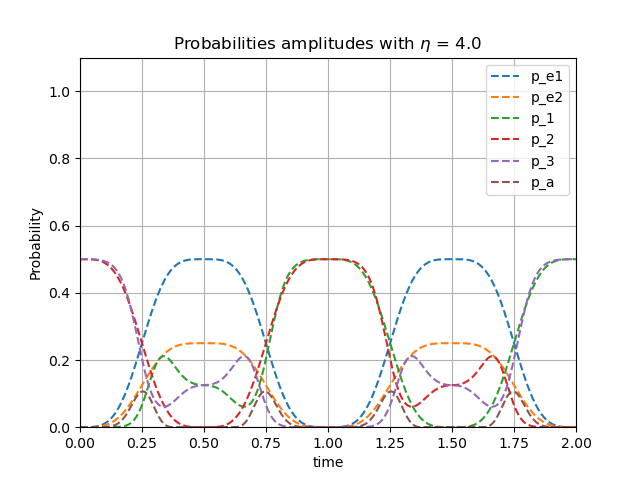
\includegraphics[scale=0.5]{figures/pop_plot_X011.png}
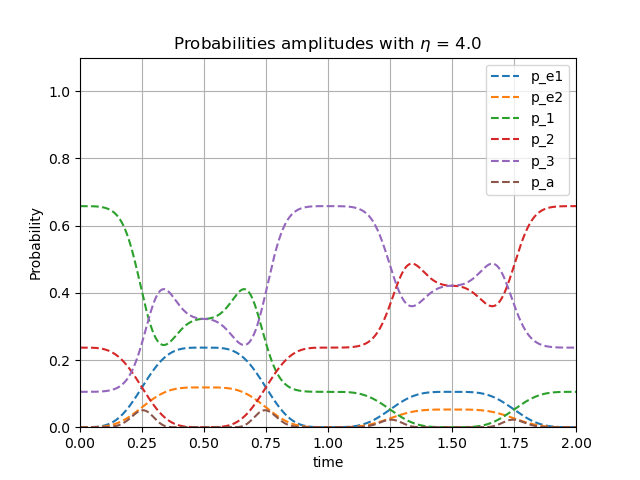
\includegraphics[scale=0.5]{figures/pop_plot_X532.png}
\caption{The effect of the $X_3$-gate on the initial states $\dfrac{1}{\sqrt{2}}[0,1,1]$ (left) and $\dfrac{1}{\sqrt{38}}[5,3,2]$ (right). Note that since the plot shows the probabilities, phases cannot be seen in the plot.}
\end{figure}

\begin{figure}[H]
\label{fig:pop_H}
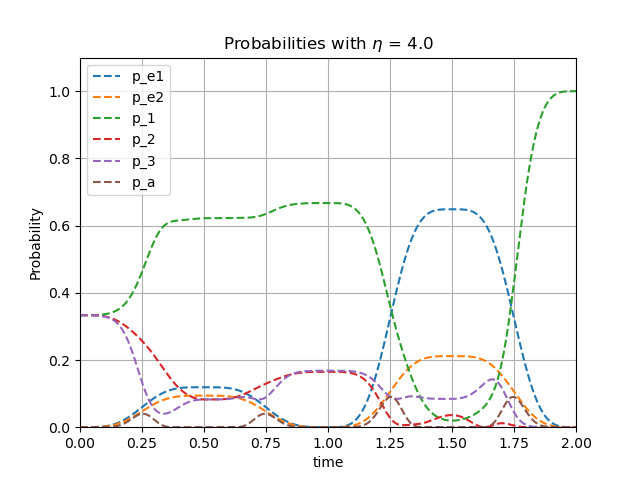
\includegraphics[scale=0.5]{figures/pop_plot_H111.png}
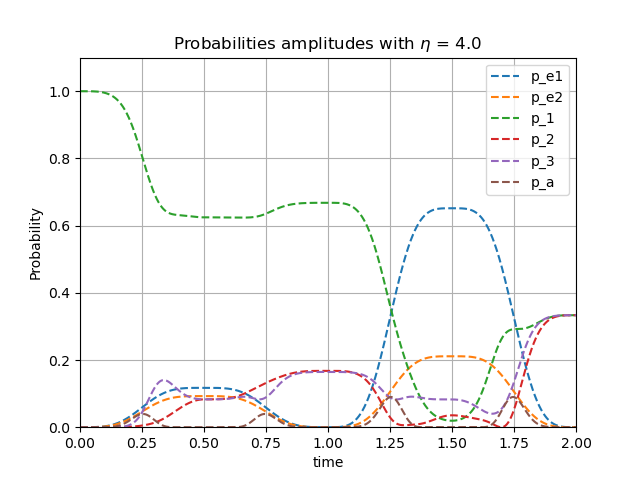
\includegraphics[scale=0.5]{figures/pop_plot_H100.png}
\caption{The effect of the $H_3$-gate on the initial states $\dfrac{1}{\sqrt{3}}[1,1,1]$ (left) and $[1,0,0]$ (right). Note that since the plot shows the probabilities, phases cannot be seen in the plot.}
\end{figure}


\subsection{Important gates, Universality and parameter selection}
By specifying the parameters of $U$ the qutrit gates from the Background section can be constructed, a selection of important gates are obtained by the following;
\begin{equation}
\begin{aligned}
X_3 &= U(0,0,\dfrac{\pi}{4},\dfrac{\pi}{2},0,\pi)U(0,0,\dfrac{\pi}{2},\dfrac{\pi}{4},0,\pi) 
= \begin{pmatrix}
0&0&1
\\
1&0&0
\\
0&1&0
\end{pmatrix}
\\ 
Z_3 &= U(0,0,0,0,\dfrac{2\pi}{3},\dfrac{4\pi}{3})
= \begin{pmatrix}
1&0&0
\\
0&e^{\frac{2\pi i}{3}}&0
\\
0&0&e^{\frac{4\pi i}{3}}
\end{pmatrix}
\\
T_3 &= U(0,0,0,0,\dfrac{2\pi}{9},\dfrac{-2\pi}{9})
= \begin{pmatrix}
1&0&0
\\
0&e^{\frac{2\pi i}{9}}&0
\\
0&0&e^{\frac{-2\pi i}{9}}
\end{pmatrix}
\\
H_3 &= U(6.41010859\cdot 10^{-4}, 6.55568952\cdot 10^{-4}, .475667128, .785362474, 1.58054108, 1.56302702)\\ \times &U(9.81289849\cdot 10^{-3}, 3.56878815\cdot 10^{-18},1.18743379, 2.15063745, 9.74301696\cdot 10^{-17}, 1.56882773)\\
&\approx \dfrac{1}{\sqrt{3}}\begin{pmatrix}
1&1&1
\\
1&e^{\frac{2\pi i}{3}}&e^{\frac{4\pi i}{3}}
\\
1&e^{\frac{4\pi i}{3}}&e^{\frac{2\pi i}{3}}
\end{pmatrix}.
\end{aligned}
\end{equation}
\note{Include calc to show $X_3$ cant be done in one loop}
Note that the choice of parameters is not unique and there are multiple ways to create the same unitary. These gates are enough to achieve single-qutrit universality as discussed in Section Theoretical Background. To achieve full universality an additional two-qutrit gate is needed. A common choice for qubits is the {\tt CNOT} gate\cite{qudit}.

The parameters for a given gate can be specified by solving the non-linear system of equations obtained from by setting the matrix representation of the gate equal to Equation \ref{eq:trit-gate-1-loop} or \ref{eq:trit-gate-2-loop}. For the diagonal gates the analytical solution can be easily found by fixing $\theta = \varphi = \chi = \xi = 0$ the basis states reduce to $\ket{d} = \ket{1}, \ket{b_1} = \ket{2}, \ket{b_2} = -\ket{3}$, then all diagonal unitaries can be specified by $\gamma_1$ and $\gamma_2$ up to a phase factor,
\begin{equation}
U(0,0,0,0,\gamma_1,\gamma_2) = \begin{pmatrix}
1&0&0
\\
0&e^{i\gamma_1}&0
\\
0&0&e^{i\gamma_2}
\end{pmatrix}.
\end{equation}

Analytical solutions are not always easy to find, the $H_3$-gate gives rise to a system of equation that is non-trivial to solve. In that case an approximative gate $\tilde{U}$ can be found by numerical optimization of the expression $\text{min}||U-\tilde{U}||_F$, where $||\cdot||_F$ is the Frobenius matrix norm given by $||A||_F = \sqrt{\text{Tr}\left[A^\dagger A \right]}$. Since $\tilde{U} \approx U$ the approximated gates effect will be very close to that of the exact gate.

To assess the robustness of the gate the fidelity is used, a metric that measures how close two quantum states are to each other, $F(\ket{\psi},\ket{\varphi}) = |\bra{\psi}\ket{\varphi}|$. The fidelity is averaged by sampling initial states and letting them evolve with time (numerically solving the Schrödinger Equation), and then comparing to the exact solution obtained by multiplying the gate with the initial state. The calculated fidelities are shown in Figure \ref{fig:fidelity}. We see that the coupling with the auxiliary state is more resilient to errors in the parameters than the original NHQC scheme. This is very similar to the results in 2 dimensions from \cite{darkpath}. Which suggests an improvement of robustness even in higher dimensions.

\begin{figure}[H]
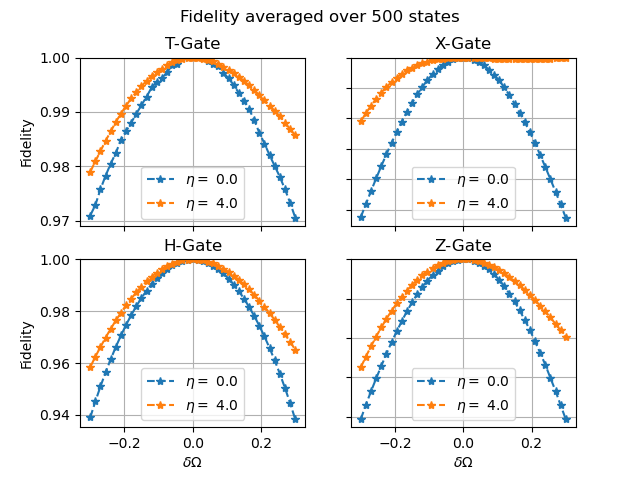
\includegraphics[scale=1]{figures/Fid500.png}

\caption{Robustness test, average fidelity of the $T_3,X_3,Z_3,$ and $H_3$ gates. Average calculated by sampling over 500 randomized initial states with a perturbation of the $\Omega$-pulses, $\Omega \mapsto \Omega(1+\delta)$ .}
\label{fig:fidelity}
\end{figure}

\section{Generalization}
To generalize the scheme to a qudit with arbitrary dimension $n$,  the same idea from the qutrit case can be extended, $n$ ground states, $m = n - 1$ excited states and 1 auxiliary state, therefore the dimension of the Hilbert space is  $n + m + 1 = n + 1 -1 = 2n$. Once again the couplings are not trivial and will be somewhat intricate, but the couplings given by the Hamiltonian in Equation \ref{eq:HamN}, will do the trick. 

\begin{equation}
H = \sum_{j = 1}^m \sum_{i = j}^n \omega_{ij} \ket{i}\bra{e_j} + \frac{\Omega_a(t)}{2}\ket{a}\bra{e_m} +\;\text{h.c}
\label{eq:HamN}
\end{equation}

\begin{figure}[H]
    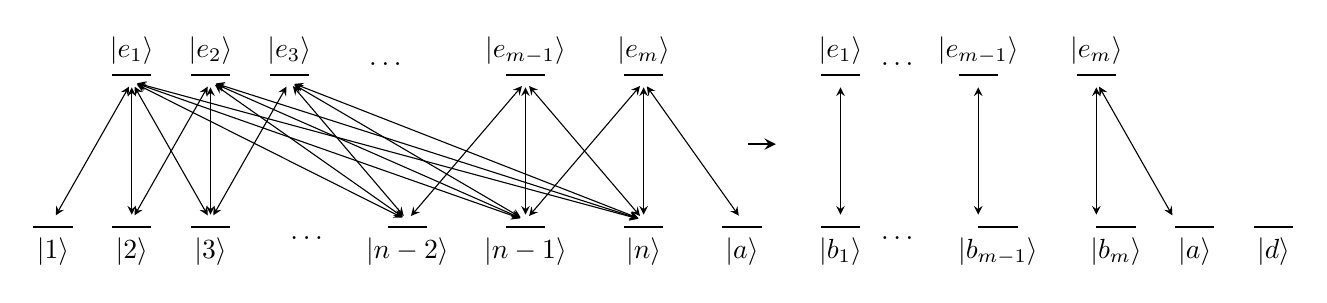
\begin{tikzpicture}[
      scale=0.5,
      level/.style={thick},
      virtual/.style={thick,densely dashed},
      trans/.style={thin,<->,shorten >=2pt,shorten <=2pt,>=stealth},
      arrow/.style={thick,->,shorten >=2pt,shorten <=2pt,>=stealth},
      classical/.style={thin,double,<->,shorten >=4pt,shorten <=4pt,>=stealth}]
    \draw[level] (4cm,-11em) -- (5cm,-11em) node[midway,below] {$\ket{1}$};
    \draw[level] (6cm,-11em) -- (7cm,-11em) node[midway,below] {$\ket{2}$};
    \draw[level] (8cm,-11em) -- (9cm,-11em) node[midway,below] {$\ket{3}$};
    \draw (11cm,-11em)  node[below] {$\dots$}; 
    \draw[level] (13cm,-11em) -- (14cm,-11em) node[midway,below] {$\ket{n-2}$};
    \draw[level] (16cm,-11em) -- (17cm,-11em) node[midway,below] {$\ket{n-1}$};
    \draw[level] (19cm,-11em) -- (20cm,-11em) node[midway,below] {$\ket{n}$};
    \draw[level] (21.5cm,-11em) -- (22.5cm,-11em) node[midway,below] {$\ket{a}$}; 
  % Draw the energy levels.
    \draw[level] (6cm,0em) -- (7cm,0em) node[midway,above] {$\ket{e_1}$};    
   	\draw[level] (8cm,0em) -- (9cm,0em) node[midway,above] {$\ket{e_2}$};
   	\draw[level] (10cm,0em) -- (11cm,0em) node[midway,above] {$\ket{e_3}$};
    \draw (13cm, 0em) node[above] {$\dots$}; 
    \draw[level] (16cm,0em) -- (17cm,0em) node[midway,above] {$\ket{e_{m-1}}$};
    \draw[level] (19cm,0em) -- (20cm,0em) node[midway,above] {$\ket{e_{m}}$};
    % Draw the transitions.
   % e_1
    \draw[trans] (6.5cm,-0.5em) -- (4.5cm,-10.5em) node[midway,left] {};
    \draw[trans] (6.5cm,-0.5em) -- (6.5cm,-10.5em) node[midway,left] {};
    \draw[trans] (6.5cm,-0.5em) -- (8.5cm,-10.5em) node[midway,left] {};
    \draw[trans] (6.5cm,-0.5em) -- (13.5cm,-10.5em) node[midway,left] {};
	\draw[trans] (6.5cm,-0.5em) -- (16.5cm,-10.5em) node[midway,left] {};
    \draw[trans] (6.5cm,-0.5em) -- (19.5cm,-10.5em) node[midway,left] {};       
   % e_2
    \draw[trans] (8.5cm,-0.5em) -- (6.5cm,-10.5em) node[midway,left] {};
    \draw[trans] (8.5cm,-0.5em) -- (8.5cm,-10.5em) node[midway,left] {};
    \draw[trans] (8.5cm,-0.5em) -- (13.5cm,-10.5em) node[midway,left] {};
	\draw[trans] (8.5cm,-0.5em) -- (16.5cm,-10.5em) node[midway,left] {};
    \draw[trans] (8.5cm,-0.5em) -- (19.5cm,-10.5em) node[midway,left] {};
    % e_3
    \draw[trans] (10.5cm,-0.5em) -- (8.5cm,-10.5em) node[midway,left] {};
    \draw[trans] (10.5cm,-0.5em) -- (13.5cm,-10.5em) node[midway,left] {};
	\draw[trans] (10.5cm,-0.5em) -- (16.5cm,-10.5em) node[midway,left] {};
    \draw[trans] (10.5cm,-0.5em) -- (19.5cm,-10.5em) node[midway,left] {};
	% e_m-1
	\draw[trans] (16.5cm,-0.5em) -- (13.5cm,-10.5em) node[midway,left] {};
	\draw[trans] (16.5cm,-0.5em) -- (16.5cm,-10.5em) node[midway,left] {};
   	\draw[trans] (16.5cm,-0.5em) -- (19.5cm,-10.5em) node[midway,left] {};
	% e_m
	\draw[trans] (19.5cm,-0.5em) -- (16.5cm,-10.5em) node[midway,left] {};
   	\draw[trans] (19.5cm,-0.5em) -- (19.5cm,-10.5em) node[midway,left] {};   			 
   	\draw[trans] (19.5cm,-0.5em) -- (22cm,-10.5em) node[midway,left] {};
   	
   	
   	
   	 \draw[arrow] (22cm,-5em) -- (23cm,-5em) node[] {}; 
   	
   	\draw[level] (24cm,-11em) -- (25cm,-11em) node[midway,below] {$\ket{b_1}$};
    \draw (26cm,-11em)  node[below] {$\dots$};    
    \draw[level] (28cm,-11em) -- (29cm,-11em) node[midway,below] {$\ket{b_{m-1}}$};
    \draw[level] (31cm,-11em) -- (32cm,-11em) node[midway,below] {$\ket{b_m}$};
    \draw[level] (33cm,-11em) -- (34cm,-11em) node[midway,below] {$\ket{a}$};
    \draw[level] (35cm,-11em) -- (36cm,-11em) node[midway,below] {$\ket{d}$};
    
  % Draw the energy levels.
    \draw[level] (24cm,0em) -- (25cm,0em) node[midway,above] {$\ket{e_1}$};    
    \draw (26cm, 0em) node[above] {$\dots$};
    \draw[level] (27.5cm,0em) -- (28.5cm,0em) node[midway,above] {$\ket{e_{m-1}}$};
    \draw[level] (30.5cm,0em) -- (31.5cm,0em) node[midway,above] {$\ket{e_{m}}$};
        
    % Draw the transitions.
   % e_1
    \draw[trans] (24.5cm,-0.5em) -- (24.5cm,-10.5em) node[midway,left] {};     
	% e_m-1
	\draw[trans] (28cm,-0.5em) -- (28cm,-10.5em) node[midway,left] {};
	% e_m
	\draw[trans] (31cm,-0.5em) -- (31cm,-10.5em) node[midway,left] {};
	\draw[trans] (31cm,-0.5em) -- (33cm,-10.5em) node[midway,left] {};
    \end{tikzpicture}
    \caption{The system given by the Hamiltonian shown in Equation \ref{eq:HamN} (left) and the transformed system from Equation \ref{eq:HamdN} (right)}
    \label{fig:HamN}
\end{figure}



The general system for a qudit is given by $m$ excited states $\ket{e_i},\,i = 0,1,\dots,m$ and $n$ ground states labeled $\ket{i},\,i = 1,2,\dots,n$ and one auxiliary state $\ket{a}$. The number of states always follows that $n-m = 1$ to limit the number of dark states to one\cite{lambda}.
The transitions occur only between excited states and ground states. The couplings follow a pattern, the first excited state $e_1$ is connected to all ground states, $e_2$ is connected to all ground states except $\ket{1}$, in general, the excited state $\ket{e_i}$ is connected to the $(n - i)$th ground states with the largest index. Unless $i = m$, the excited state $\ket{e_m}$ is connected to the two highest labeled ground states and the auxiliary state $\ket{a}$. See Equation \ref{eq:HamN} and Figure \ref{fig:HamN} for a clarification. 

From the standard basis $\{e_1,e_2,\dots,e_m,1,2,\dots,n,a\}$, it is possible define a new basis, the dark state basis given by $\{e_1,e_2,\dots,e_m,b_1,b_2,\dots,b_{m},a,d\}$.

Assume there exists a dark state on the form 
\begin{equation}
\ket{d} = c_1\ket{1} + c_2\ket{2} + c_3\ket{3} \dots + c_{n}\ket{n},\, |c_1|^2 + |c_2|^2 + \dots + |c_{n}|^2 = 1
\end{equation}
from this dark state one could define $n-1 = m$ bright states. Starting from $\ket{b_1}$, constructing it such that it will be orthogonal to the dark state and all other bright states,
\begin{equation}
\ket{b_1} = N_1\left(-c_2^{*}\ket{1} + c_1^{*}\ket{2}\right)
\end{equation}
with $N_1$ being a normalization factor. Then choose additional bright states are on the form
\begin{equation}
\label{eq:birght_states}
\begin{aligned}
&\ket{b_2} &=& N_2 \left(c_1\ket{1} + c_2\ket{2} + \Lambda_3\ket{3}  \right)
\\
&\ket{b_3} &=&  N_3 \left(c_1\ket{1} + c_2\ket{2} + c_3\ket{3} + \Lambda_{4}\ket{4} \right)
\\
&\;\;\vdots
\\
&\ket{b_{m-1}} &=& N_{m-1} \left( c_1\ket{1} + c_2\ket{2} + c_3\ket{3}  + \dots + c_{m-1}\ket{m-1}+ \Lambda_m\ket{m} \right)
\\
&\ket{b_{m}} &=& N_m \left( c_1\ket{1} + c_2\ket{2} + c_3\ket{3}  + \dots + c_m\ket{m} + \Lambda_{m+1}\ket{m+1} \right).
\end{aligned}
\end{equation}
By construction,  $\ket{b_1}$ is orthogonal to the dark state  all other bright states. for $k \geq 2$ $\ket{b_k}$ is $k+1$-dimensional, so it consists of $k+1$ basis-kets, where the coefficient in front of the last ket, $\Lambda_{k+1}$ is chosen such that $\ket{b_k}$ is orthogonal the dark state, $\ket{d}$. This will in turn make $\ket{b_k}$ orthonormal to any $\ket{b_{>k}}$ as they have the same states and coefficients as $\ket{d}$ for all the states involved in the inner product $\bra{b_{>k}}\ket{b_k} = \bra{d}\ket{b_k}$. Therefor by chosing $\Lambda_k$ such that these inner product are zero the construction will results in orthonormal states,  $\bra{b_i}\ket{b_j} = \delta_{ij}$. Explicitly for the state $\ket{b_{k}}$,$k \geq 2$, the coefficient $\Lambda_k+1$ will be given by 
\begin{equation}
\Lambda_{k+1} = -\dfrac{1}{c_{k+1}^{*}}\sum_{l = 1}^{k}|c_l|^2
\end{equation}
and the normalization $N_{k}$ is given by 
\begin{equation}
N_k =  \left( \sum_{l = 1}^k|c_l|^2  + \left|\Lambda_{k+1}\right|^2 \right)^{-1/2} = \left( \sum_{l = 1}^k|c_l|^2  + \left|-\frac{1}{c_{k+1}^{*}}\sum_{l = 1}^{k} |c_l|^2 \right|^2 \right)^{-1/2}
\end{equation}


The coefficients $c_i$ can be parametrized by the euclidean components of the radius of the unit-$n$-sphere with an added phase factor.

\begin{equation}
\begin{aligned}
c_1 &= \cos(\varphi_1)
\\ 
c_2 &= e^{i\theta_1}\sin(\varphi_1)\cos(\varphi_2)
\\ 
c_3 &= e^{i\theta_2}\sin(\varphi_1)\sin(\varphi_2)\cos(\varphi_3)
\\
&\hspace{2mm}\vdots
\\
c_{n-1} &= e^{i\theta_{n-1}}\sin(\varphi_1)\dots\sin(\varphi_{n-2})\cos(\varphi_{n-1})
\\
c_{n} &= e^{i\theta_{n}}\sin(\varphi_1)\dots\sin(\varphi_{n-2})\sin(\varphi_{n-1})
\end{aligned}
\end{equation}

$c_1$ does not need a phase factor since the overall phase of a state is non-measurable and can be chosen such that the first phase factor will cancel out. 

In this newly defined space, the Hamiltonian can be written as
\begin{equation}
H_d = \sum_{i = 1}^m \frac{\Omega_i(t)}{2}e^{-i\phi_i}\ket{b_i}\bra{e_i} + \frac{\Omega_a(t)}{2}\ket{a}\bra{e_m} +\;\text{h.c}
\label{eq:HamdN}
\end{equation}
with $\Omega_i$ being real-valued time dependent parameters and the $\phi_i$ time independent phase factors. The explicit transformation from $H \mapsto H_d$ is not that important but could be obtained by expanding the bright state kets into the standard basis from (\ref{eq:birght_states})

With this Hamiltonian $m$ independent dark paths can be constructed, and must satisfy $\bra{D_i(t)}H_d\ket{D_i(t)} = 0, i = 1,2,\dots,m$ and $\bra{D_i(t)}\ket{D_j(t)} = \delta_{ij}$.\\
The dark paths can be parametrized by two functions $u(t),v(t)$ that satisfy the conditions $u(0) = v(0) = u(T) = v(T) = 0$,  will have the form
\begin{equation}
\begin{aligned}
\ket{D_i(t)} &= \cos u e^{-i\phi_i}\ket{b_i} + i\sin u \ket{e_i},\, i = 1,2,\dots,m-1
\\
\ket{D_m(t)} &= \cos u \cos v e^{-i\phi_n}\ket{b_m} - i\sin u \ket{e_m} - \cos u \sin v \ket{a}
\end{aligned}
\end{equation}
The dark paths start in the bright state and travel along a curve where the expectation value of the energy is constantly $0$ and can thus be used non-adiabatically.

By using these states one can reverse engineer the Hamiltonian using the Schrödinger equation to determine $\Omega_i$ and $\Omega_a$ since 
\begin{equation}
i\pdv{}{t}\ket{D_i(t)} = H_d\ket{D_i(t)},\; i = 1,2,\dots,m
\end{equation}
a calculation yields
\begin{equation}
\begin{aligned}
\Omega_1(t) &= -2\dot{u}
\\ 
\Omega_2(t) &= -2\dot{u}
\\
&\hspace{2mm}\vdots
\\
\Omega_{m-1}(t) &= -2\dot{u}
\\
\Omega_m(t) &= 2\left(\dot{v}\cot u\sin v + \dot{u}\cos v \right)
\\
\Omega_a(t) &= 2\left(\dot{v}\cot u\cos v - \dot{u}\sin v \right)
\end{aligned}
\end{equation}

The time evolution is split into $k$ loops, each loop with two pulses, $0 \longrightarrow T/2$ and $T/2 \longrightarrow T$. The relevant part of the time evolution operator for one loop is  
$U_1(T/2,0) = \ket{d}\bra{d} -i\sum_{i = 1}^m \ket{e_i}\bra{b_i},\, \phi_i = 0, i = 1,2,\dots,n$ and $U_2(T,T/2) = \ket{d}\bra{d} + i\sum_{i = 1}^m e^{i\gamma_i}\ket{b_i}\bra{e_i},\, \phi_i = 0, i = 1,2,\dots,n $
The full operator for one loop is then given by 
\begin{equation}
U = U_2U_1 = \ket{d}\bra{d} + \sum_{i = 1}^{m}e^{i\gamma_i}\ket{b_i}\bra{b_i}.
\end{equation}
It is clear that $U$ is unitary in the subspace $\{d,b_1,b_2,\dots, b_n\}$

The unitary is parametrized by $3m = 3(n-1), n\geq 2$, parameters,
\begin{equation}
U(\varphi_1,\dots,\varphi_m,\theta_1,\dots,\theta_m,\gamma_1,\dots,\gamma_m) 
\end{equation} 

Applying the unitary with different parameters in sequence up to $k$ times is enough to create any desirable gate $\mathcal{U} = U^k$. The unitary is controlled by $3(n-1)$ parameters while $n$ dimensional qudit has more degrees of freedom than covered with a single loop.

The qudit state space is equivalent to $SU(n)$, which has dimensionality $\dim(SU(n)) = n^2 -1$. To cover all degrees of freedom $k$ must satisfy $3(n-1)k \geq n^2 -1$.
which means $k \geq \frac{n+1}{3}$. Thus the number of loops needed to create any unitary scales linearly at worst since some gates can be created with fewer loops, see Table \ref{tab:dim}. 

In the case of equality $k =\frac{n+1}{3}$, when $n = 3j + 2,\, j \in \mathbb{N}$, the fewest amount of loops per dimension is achieved and could potentially be more efficient carriers of information since the same number of loops must be carried out while higher dimension has higher information capacity.

\begin{table}[H]
\centering 
\begin{tabular}{|c|c|c|c|c|}
\hline
$n$ & $3(n-1)$ & $n^2 - 1$ & $k$ &  '='\\
\hline
2& 3& 3& 1& \checkmark \\
3& 6& 8& 2& \\
4& 9& 15& 2& \\
5& 12& 24& 2& \checkmark \\
6& 15& 35& 3& \\
7& 18& 48& 3& \\
8& 21& 63& 3& \checkmark \\
9& 24& 80& 4& \\
10& 27& 99& 4& \\
11& 30& 120& 4& \checkmark \\
12& 33& 143& 5& \\
\hline
\end{tabular}
\caption{Table for some dimensions.}
\label{tab:dim}
\end{table}

The scaling of the qudit gate is linear at worst both in the number of loops and the number of parameters needed for control. In fact, any diagonal gate only requires one loop, by setting $\varphi_1 = \dots \varphi_m = \theta_1 = \dots = \theta_m = 0$ the unitary reduces to the form
\begin{equation}
\label{eq:diagate}
U(0,\dots,0,\gamma_1,\dots,\gamma_m) = \ket{1}\bra{1} + \sum_{k = 2}^n e^{i\gamma_k}\ket{k}\bra{k}.
\end{equation}
The effect of this variable choice makes $c_1 = 1, c_{i\neq 1} = 0$. By (\ref{eq:birght_states}) the only thing not clear is how this affects the $\Lambda$ coefficients.
For the state $\ket{b_k}$, $k \geq 3$, fixing $c_1 = 1$ and let all other states approach $0$.
\begin{equation}
\begin{aligned}
\lim_{c_{i\neq 1} \rightarrow 0} \ket{b_k} &= \lim_{c_{i\neq 1} \rightarrow 0}\frac{1}{N_k}\Lambda_{k+1} \ket{k+1}\\
&= \lim_{c_{i\neq 1} \rightarrow 0} \left(1  + \left|-\frac{1}{c_{k+1}^{*}}\right|^2 \right)^{-1/2}\left(-\frac{1}{c_{k+1}^{*}}\right) \ket{k+1} \\
&= \lim_{c_{i\neq 1} \rightarrow 0} \left|-\frac{1}{c_{k+1}^{*}}\right|^{-1}\left(-\frac{1}{c_{k+1}^{*}}\right) \ket{k+1} \\
& = -\ket{k+1}
\end{aligned}
\end{equation}
Therefor $\ket{d} = \ket{1}, \ket{b_1} = \ket{2}, \ket{b_2} = -\ket{3}, \ket{b_3} = -\ket{4}, \dots, \ket{b_m} = -\ket{m+1}$, and thus the unitary will take the form (\ref{eq:diagate}) so any diagonal unitary can be created up to any unimportant phase.

Thusly, any phase flip gate, such as $Z_n$ can be constructed in any dimension using only one loop. Since the gates essential for single-quidit universality is $\{T_n, H_n\}$, where one of the gates can be obtained by a single loop. Thus only the Hadamard gate will be the most costly part of the scheme as it requires at most $k = \frac{n+1}{3}$ loops in $n$ dimensions. Since the $T_n$ gate only is defined for prime $n$ the dimensions of greatest interest will be the prime dimensions where $3(n-1)k = n^2 -1$. Since these seems to be the most information carrying with the fewest number of loops where universality could be implemented. The first few of these perfect-prime dimensions are $n = 5,11,17,23,\dots$. It has already been shown that fault tolerant QC is implementable in odd prime dimensions\cite{magic-muller}, so a high fidelity controllable scheme in these dimensions would be desirable.



The quantum gate $\mathcal{U}$ can be formulated as a linear combination of the dark state and dark paths just as in the qutrit case,
\begin{equation}
\ket{\psi(t)} = f_0\ket{d} + \sum_{i = 1}^{m}f_i\ket{D_i(t)}, t \in [0,T]
\end{equation}
where the coefficients can be solved for by choosing an initial state $\ket{\psi(0)}$. This corresponds to one loop, by using $\ket{\psi(T)}$ as an initial state for the next loop. By iterating this method one can simulate $\mathbb{U} = U^k$ where each loop $U$ have a different set of parameters. So in theory this can be implemented and simulated for any dimensional qudit, just as for the case of the qutrit. 







\newpage
\section{Conclusions and outlook}
%% Conclusions
We have shown how to explicitly create a quantum mechanical system, which could be used to emulate a qutrit and corresponding single-qutrit gates. This is done by expanding the dark path qubit scheme \cite{darkpath} into a higher dimension. We have shown how it will generalize in the qudit case and using auxiliary states to improve the robustness of the gates. Universality for the qutrit can be obtained using the Hadamard and $T$-gate equivalent gates in 3 dimensions. The qutrit gates have a high fidelity and their robustness is improved by the inclusion of the auxiliary state in a similar way as for the qubit \cite{darkpath} which suggests that this method can be beneficial for higher dimensional qudits to improve robustness. In the general case for the qudit we have also shown how any dimensional single-qudit diagonal unitary could be created by a single multi-pulse loop in parameter space and that non-diagonal unitaries scale linearly at worst in the number of loops and parameters required for control of each loop scale linearly. The possibility that the scheme expands efficiently into certain prime dimension have been discussed.
\\

%% Outlook
\noindent One of the greatest challenges of this project was how to choose parameters to replicate the unitary gates. Analytical construction of any diagonal unitary is solved, but there are many other gates that would be interesting to study in more detail. First, looking deeper into how different constraints on the parameters impact the construction of gates and vice versa. Second, how does the number of parameter space loops required relate to which unitaries are reachable. This problem is very interesting since reduction of loops decreases the number of parameters needed for control, fewer loops implies less error and makes the scheme less costly to run. For both those cases the usage of numerical optimization poses interesting problems to study. Will the numerically optimized gates perform worse than analytical ones, and are there any deeper problems associated with this method? Numerical optimization in the high dimensional parameter spaces present in these system is most likely not well-behaved and may contain a lot of false minima. There might be some structure related to the parametrization that could be used to study the parameter space to gain insight into how to optimally solve the problem.
 
Another obvious concern that could be addressed is the lack of multi-qudit gates. Entanglement is one of the fundamentals of QC and extending the scheme to include these would be an obvious improvement. This could maybe be achieved through some detuning or by some more explicit physical implementation similar to the qubit case in \cite{darkpath}.

Lastly, we have shown how to construct the qudit in any dimension but only analyzed and simulated the qutrit. With the generalization in hand, writing a script which could apply the scheme to dynamically generate qudit gates of arbitrary dimension seems quite possible. Studying the larger prime dimensions to compare efficiency and check fidelity of the gates would be interesting to look into more.

Overall many aspects would be interesting to delve deeper into, and I am almost certain that improvements to this scheme would be possible.



\newpage
\bibliographystyle{vancouver}
\bibliography{ref.bib}
\newpage

\appendix

\section{Code}
\note{Kod här}
\end{document}